\documentclass[sigplan]{acmart}
\AtBeginDocument{%
  \providecommand\BibTeX{{%
    Bib\TeX}}}

\usepackage{minted}

\acmConference[DSC148]{Final Project}{March, 2023}{La Jolla, California, USA}

\title{Loan Predictions DSC148 Final Project Report}

\begin{document}
\author{Jack Kai Lim}
\authornote{Both authors contributed equally to this research.}
\affiliation{%
    \institution{University of California, San Diego}
    \city{San Diego}
    \country{United States}
}
\email{jklim@ucsd.edu}

\author{Shrishti Seksaria}
\authornote{Both authors contributed equally to this research.}
\affiliation{%
    \institution{University of California, San Diego}
    \city{San Diego}
    \country{United States}
}
\email{sseksari@ucsd.edu}


\begin{teaserfigure}
    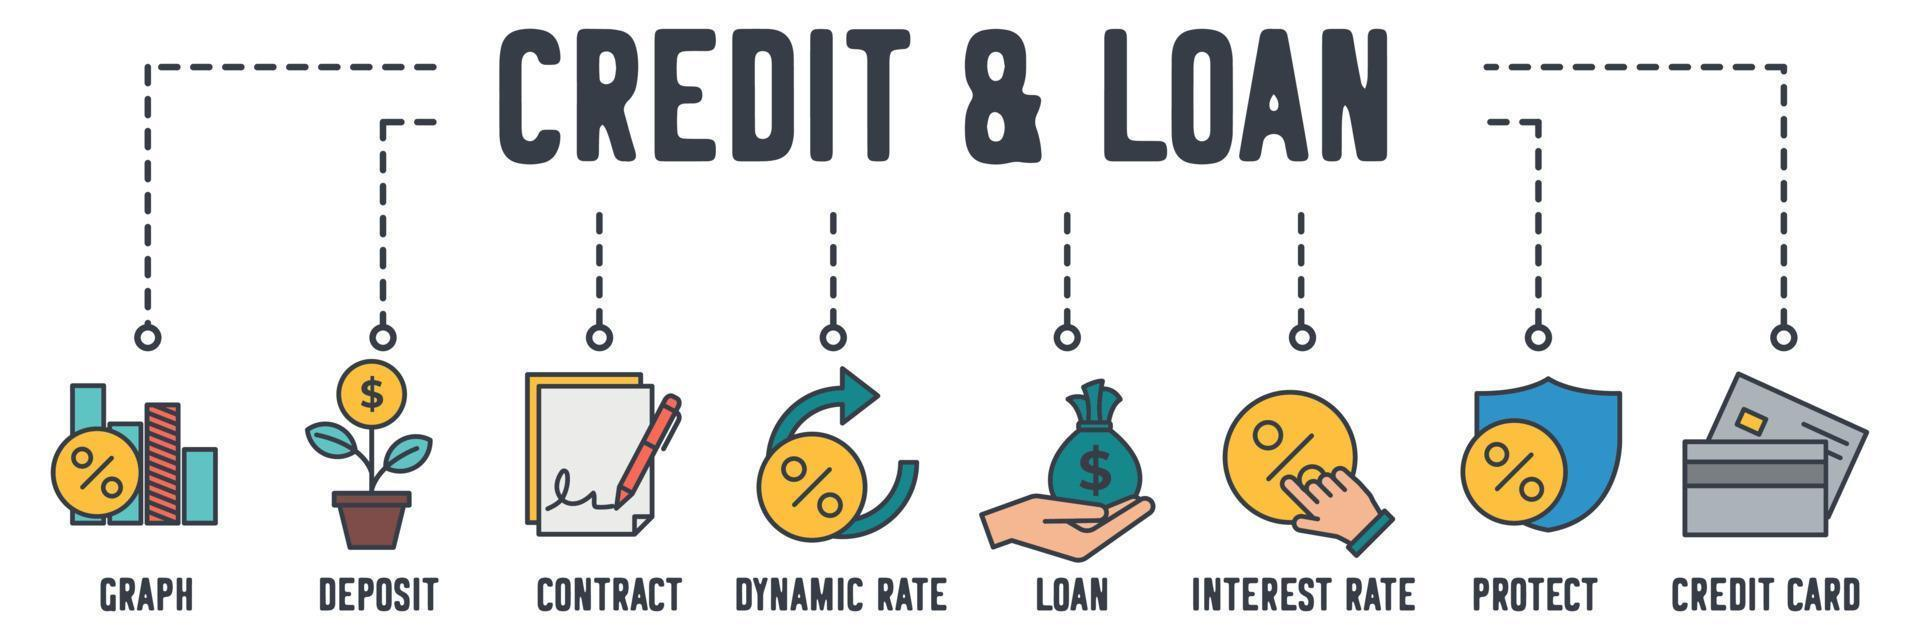
\includegraphics[width=\textwidth]{images/card banner.jpg}
    \caption{Credit Card Loans}
    \Description{3 Credit cards images}
    \label{fig:teaser}
\end{teaserfigure}



\maketitle


%-----------------------------------------------------------------------
\section{Introduction}
\label{sec:intro}
Our credit loans prediction project is centered around a comprehensive dataset that we obtained from \href{https://www.kaggle.com/datasets/hemanthsai7/loandefault}{\textbf{Kaggle}}. The dataset is specifically about predicting loan approvals, and we are using it to train a machine learning model. The goal of this project is to accurately predict the approvals based on various factors that the dataset provides.

The process of determining loans can often be a time-consuming and unreliable task. By using a machine learning model to help predict the loan approvals, we hope to find out a better and quicker way to be able to give out predictions to ones possibility of getting an approval for their credit loans. The machine learning model will take into account various factors that can affect whether a person gets approved for their loans or not.

Overall, we hope to build a well-rounded and accurate model for predicting credit loans.

\section{Dataset Description}
We are using a dataset from Kaggle called \textbf{Loan Default Prediction}. The dataset is stored in two csv files: \textbf{train.csv} and \textbf{test.csv}. The dataset has 67463 rows of data, with each row representing a loan application. There are 35 columns in the dataset, each containing information given by the applicant for the loan. We will use these features to predict whether the loan is approved or not.

To better understand the dataset, we went over all features that we did not completely understand and looked up their definitions in order to get a better understanding of what each feature tells us and their value in determining whether the loan is approved or not.

Some of the features that we looked up are:
\begin{itemize}
    \item 'Grades' and  'Subgrades'. These features are used to determine the risk in loaning an applicant, and the higher the grade and the subgrade the lower the risk.
    \item Revolving balance: The amount of debt owed on a credit card account at the end of each billing cycle. This balance can vary from month to month, depending on how much the cardholder charges and pays off.
    \item Revolving utilities: The percentage of a person's total revolving credit limit that is currently being used. This is also known as credit utilization. For example, if a person has a total credit limit of \$10,000 across all their credit cards and has a total balance of \$5,000, their revolving utilities would be 50\%.
    \item Total revolving credit limit: The maximum amount of credit that a person has available on their revolving credit accounts, such as credit cards or lines of credit. This includes the credit limits on all of a person's revolving accounts, even if they currently have a \$0 balance.
    \item Recoveries: The amount of money that has been recovered by the lender or loan servicer from a borrower who was previously delinquent on their loan payments. This can include payments made by the borrower, as well as any fees or charges that were added to the loan balance.
    \item Collection recovery fee: A fee that is charged by the lender or loan servicer when a delinquent borrower makes a payment or agrees to a repayment plan. This fee is intended to cover the costs of collection efforts and is typically a percentage of the amount that is recovered.
    \item Collection 12 month medical: A type of collection account that is related to medical debt. This may include unpaid medical bills or other medical expenses that were not covered by insurance.
    \item Total collection amount: The total amount of debt that is in collection, including both the principal balance of the loan and any fees or charges that have been added.
\end{itemize}

\section{EDA}
\subsection{Dataset Cleaning}
We conducted a thorough exploratory data analysis to determine which columns in the dataset were relevant in predicting whether a loan would be approved or not. During the cleaning process, we removed several columns that were deemed irrelevant in determining loan approval. We examined each column in the dataset to gain a better understanding of what each feature tells us and their correlation with the target variable.

The columns that were removed from the dataset include 'ID', 'Term', 'Payment Plan', 'Open Account', 'Batch Enrolled', 'Accounts Delinquent', 'Total Accounts', 'Recoveries', 'Initial List Status', 'Collection Recovery Fee', 'Last week Pay', 'Revolving Balance', 'Revolving Utilities', 'Funded Amount', 'Inquires - six months', and 'Loan Title'.

We discovered that columns such as 'ID' and 'Batch Enrolled' were unnecessary as they provided no significant information in determining whether a loan would be approved or not as unique identifiers such as ID is not important, while, Batch Enrolled is mainly used to speed up the process of approving loans hence it does not tell us any important information either.
Similarly, the columns 'Term' and 'Payment Plan' were removed from the dataset as they did not have a significant impact on whether a loan would be approved or not. We also removed 'Open Account' and 'Total Accounts' as the number of accounts a person has does not necessarily determine their financial capability or responsibility.

Furthermore, we removed 'Accounts Delinquent' as we already have the delinquency in the past two years for each applicant, which we deemed more important in predicting whether a loan would be approved or not. The columns 'Recoveries', 'Initial List Status', 'Revolving Balance', 'Revolving Utilities', 'Inquires - six months', and 'Collection Recovery Fee' were also removed as they were found to have little variation between the two classes. Based on our research, we concluded that their correlation was not high enough to keep them in the dataset to prevent overfitting.

Here is the visualization for the columns 'Recoveries', 'Initial List Status', 'Revolving Balance', and 'Inquires - six months'. The analysis showed that there was little variation between the two classes, which further supported our decision to remove these columns from the dataset.

After that we are left with these columns,
\begin{itemize}
    \item Loan Amount: The total amount of the loan
    \item Funded Amount Investor: The total amount of the loan funded by investors
    \item Interest Rate: The interest rate of the loan
    \item Grade: The loan grade of the loan
    \item Sub Grade: The loan subgrade of the loan
    \item Employment Duration: The duration of the employment of the borrower
    \item Home Ownership: The home ownership of the borrower
    \item Verification Status: The verification status of the loan
    \item Debit to Income: The ratio of the total monthly debt payments to the monthly income
    \item Delinquency - two years: The number of 30+ days past due incidences of delinquency in the borrower's credit file for the past 2 years
    \item Total Received Interest: The total amount of interest received
    \item Total Received Late Fee: The total amount of late fees received
    \item Collection 12 months Medical: The total amount of collection fees received
    \item Application Type: The application type of the loan
    \item Total Collection Amount: The total amount of collection fees received
    \item Total Current Balance: The total amount of collection fees received
    \item Total Revolving Credit Limit: The total amount of collection fees received
    \item Loan Status: The status of the loan
\end{itemize}

Please see the following graphs for a more detailed analysis on the columns that were removed from the dataset:

\begin{figure}[h]
    \centering
    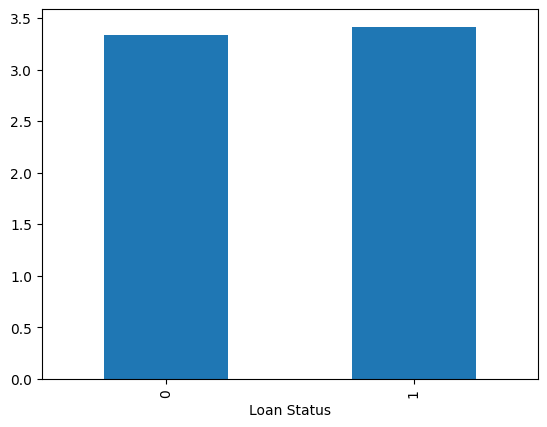
\includegraphics[width=8cm, height = 5.5cm]{images/recoveries.png}
    \caption{Recoveries Bar Chart}
    \Description{Recoveries Bar Chart}
\end{figure}

\begin{figure}[h]
    \includegraphics[width=8cm, height = 5.5cm]{images/initial list status.png}
    \caption{Initial List Status Bar Chart}
    \Description{Initial List Status Bar Chart}
\end{figure}

\begin{figure}[h]
    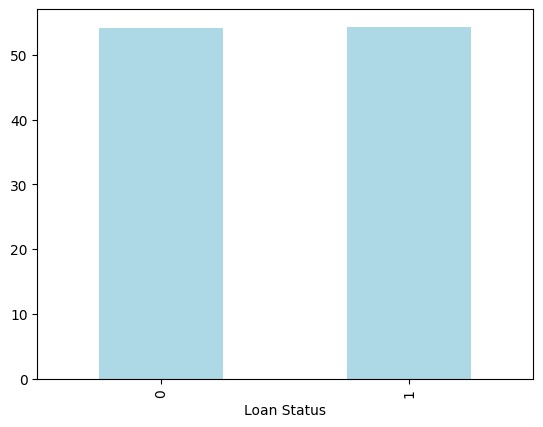
\includegraphics[width=8cm, height = 5.5cm]{images/revolving utilities.png}
    \caption{Revolving Utilities Bar Chart}
    \Description{Revolving Utilities Bar Chart}
\end{figure}

\begin{figure}[h]
    \centering
    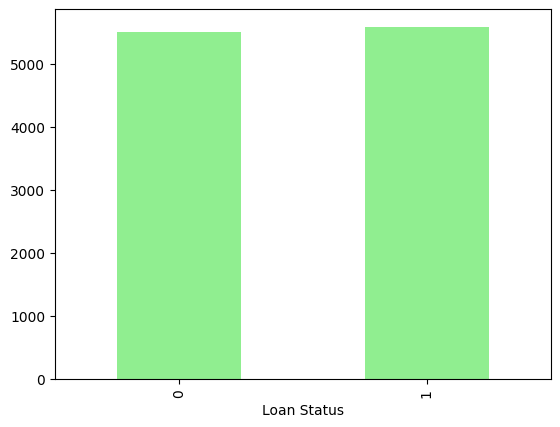
\includegraphics[width=\linewidth]{images/revolving balance.png}
    \caption{Revolving Balance Bar Chart}
    \Description{Revolving Balance Bar Chart}
\end{figure}

\begin{figure}[h]
    \includegraphics[width=\linewidth]{images/inquires six months.png}
    \caption{Inquires - Six Months Bar Chart}
    \Description{Inquires - Six Months Bar Chart}
\end{figure}

\subsection{Univariate Analysis}
\begin{figure*}[h]
    \centering
    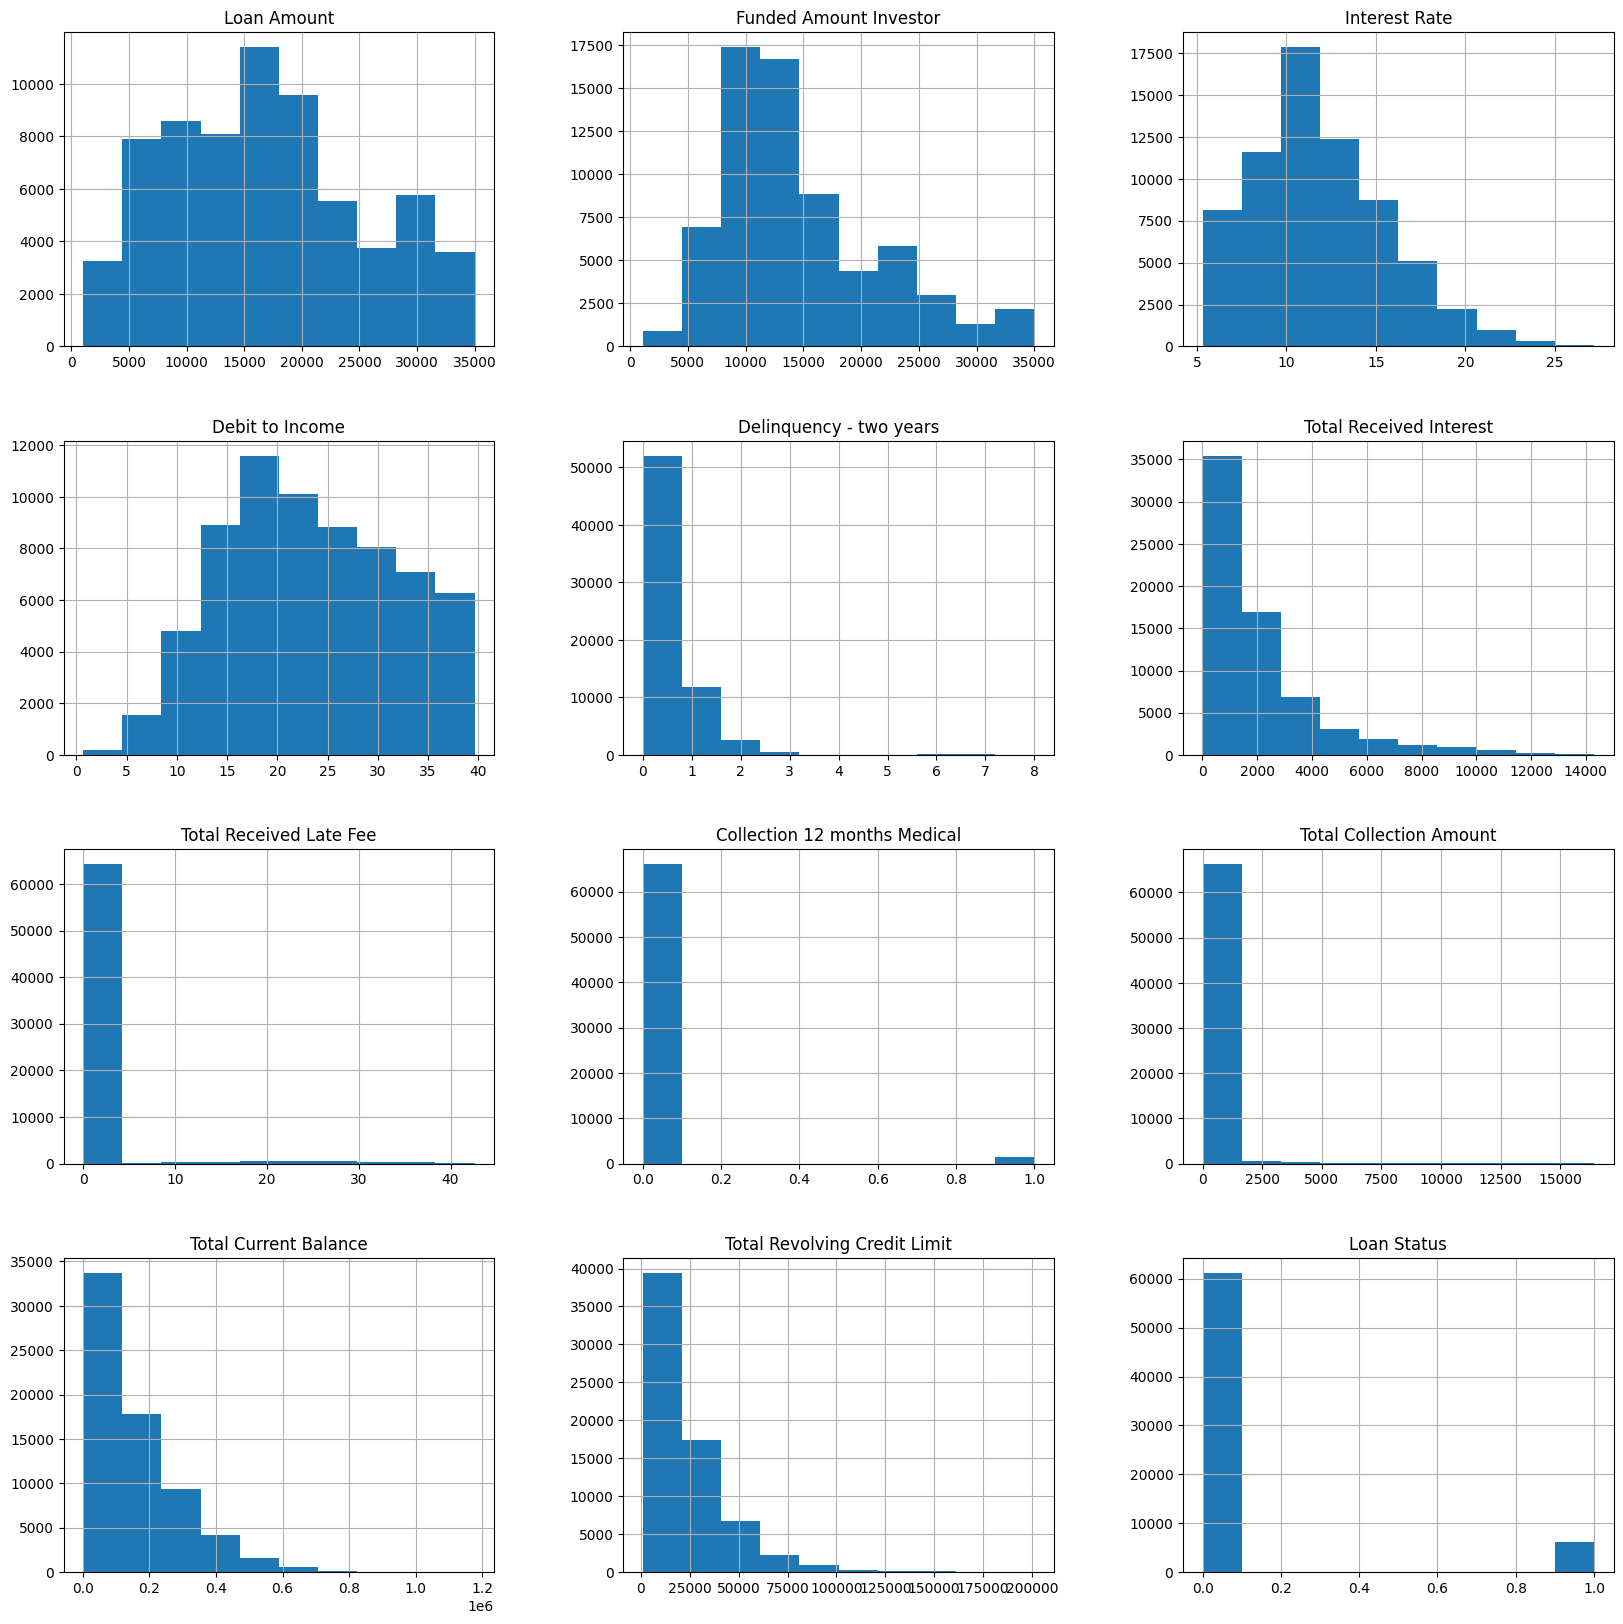
\includegraphics[width=\linewidth]{images/univariate_hist.png}
    \caption{Numerical Data Distribution}
    \Description{Numerical Data Distribution}
\end{figure*}
We begun our data analysis to look for correlation in the data byt first doing some univairate analysis.
The first thing we looked into was the distribution of the numerical data which is shown in the following graph:


Our exploratory data analysis revealed that the `Loan Status` feature has a significant discrepancy between the two classes. To reduce bias towards the 0 class when training the model, we will attempt to decrease the number of 0 classifications.

Additionally, we discovered that `Total Current Balance`, `Total Revolving Credit Limit`, `Total Collection Amount`, `Total Received Late Fee`, and `Total Received Interest` exhibit high skewness. To address this, we will attempt to reduce the skewness of these variables.

These findings will be critical in our credit loans prediction, as the skewness of the data could affect our predictions and cause unnecessary bias towards the data,
hence, I will be zoning in on these variables in order to visualize a method in which we can use to reduce the skewness of the data.

In order to reduce the weight of the outlier data affecting our predictions, I plotted a box and whisker plot in order to see comparitively how
far the outliers are from the mean of the data, which will determine whether we should standardize the feature or not.

The following are the box and whisker plots for the features `Total Current Balance`, `Total Revolving Credit Limit`, `Total Collection Amount`, `Total Received Late Fee`, and `Total Received Interest`:
\begin{figure*}[h]
    \centering
    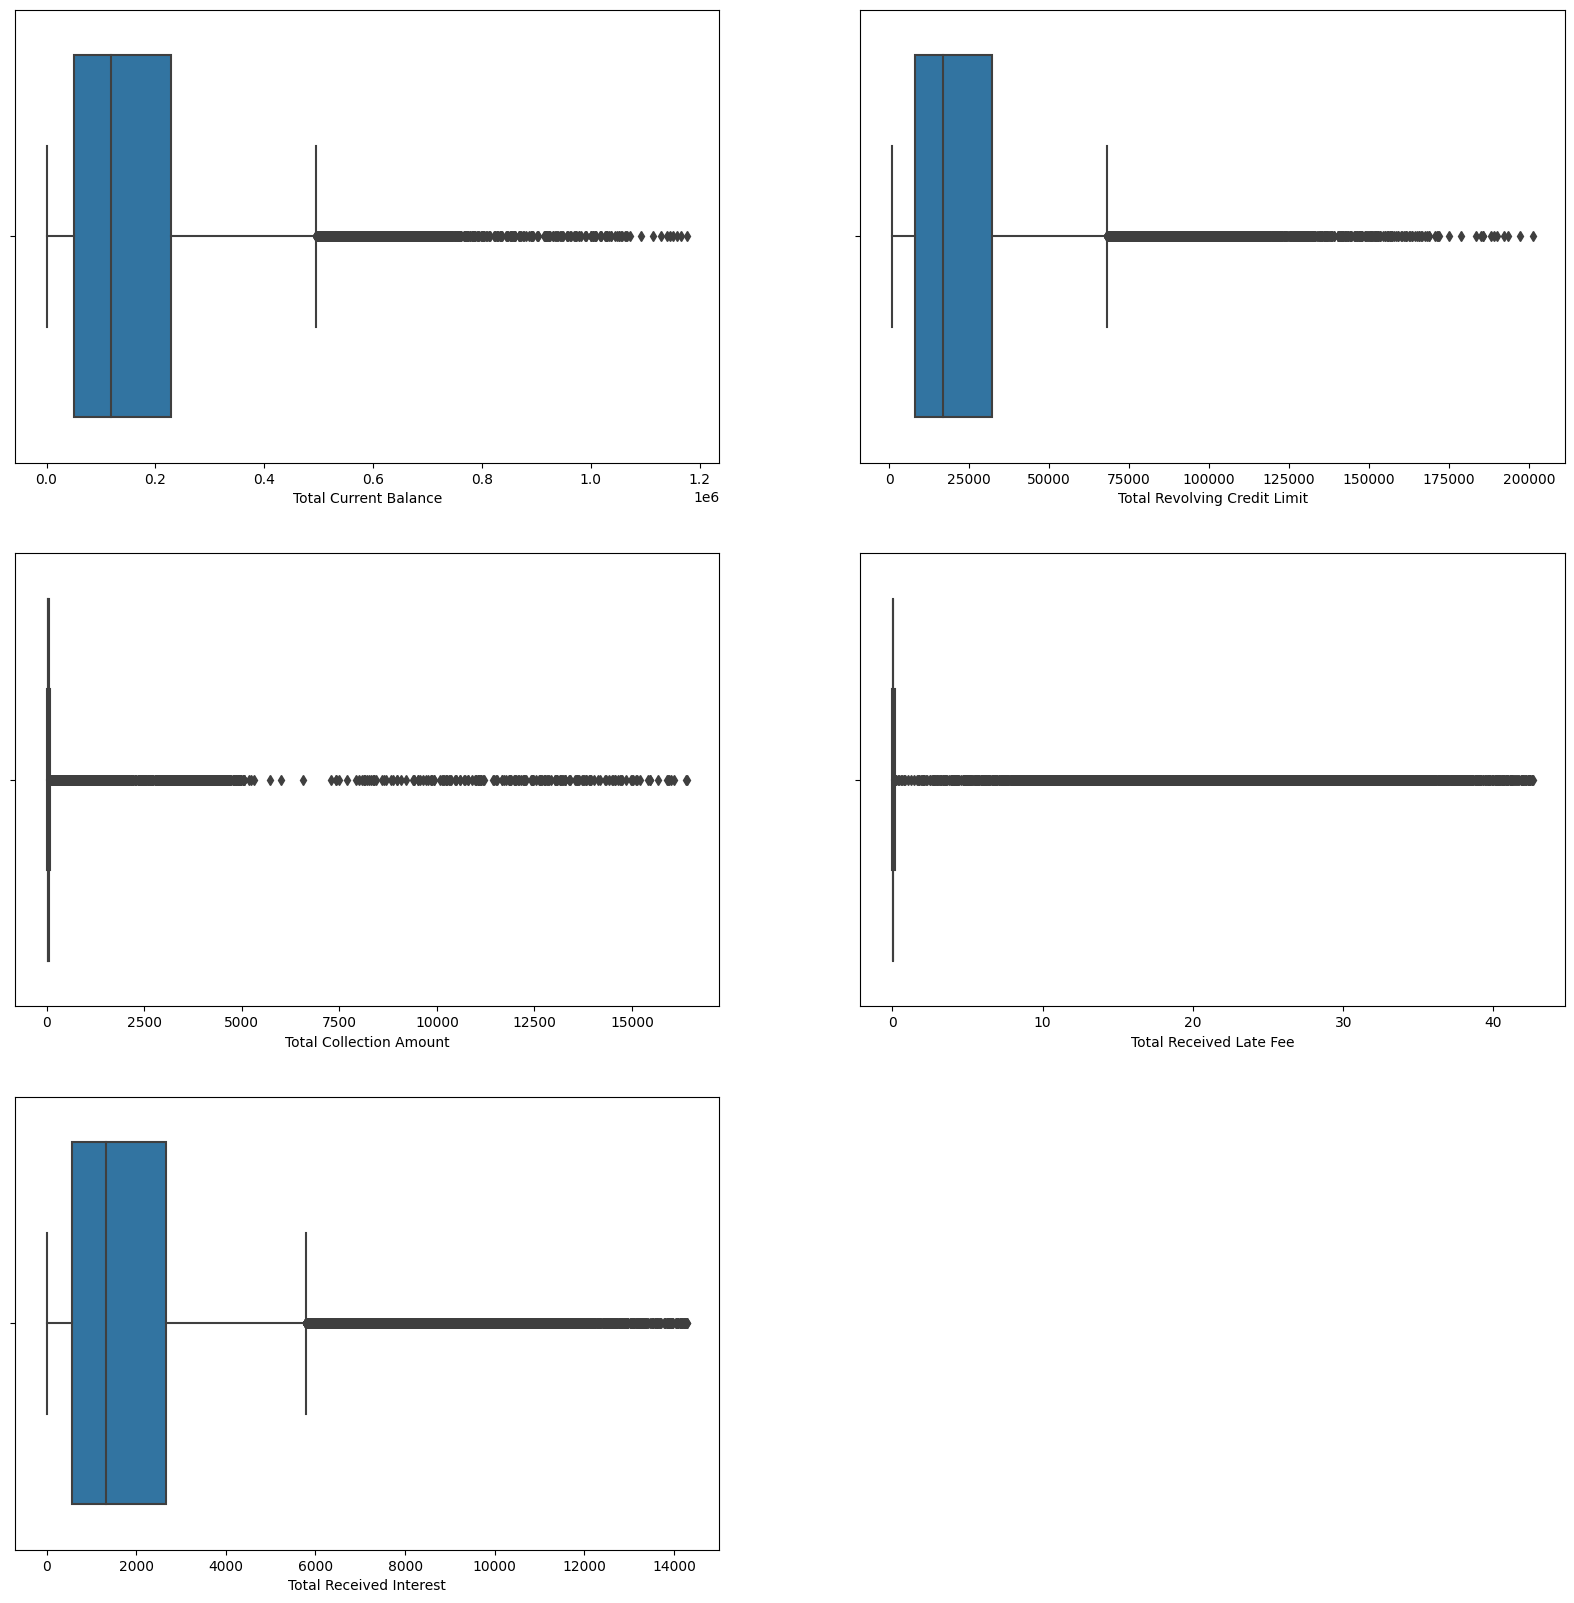
\includegraphics[width=\linewidth]{images/boxnwhiskers.png}
    \caption{Univariate Box and Whisker Plot Visualization}
    \Description{Univariate Box and Whisker Plot Visualization}
\end{figure*}
\newpage
Looking at the box and whisker plots, the features 'Total Collection Amount', 'Total Received Late Fee' are extremely skewed and have a lot of outliers. This is because the majority of the data is concentrated at the lower end of the scale, while the outliers are at the higher end of the scale.
This is a problem because the outliers will have a significant impact on the mean of the data, which will cause the model to be biased towards the outliers. Therefore, we will need to standardize these features in order to reduce the impact of the outliers on the mean of the data.

The other features on the other hand, have a lot of outliers, but are not too incredibly skewed so we may not standardize them.
\newpage
\subsection{Bivariate Analysis}
In the Bivariate Analysis, we are interested in exploring the relationship between two variables. In this case, we are looking at the correlation between a person's grades and how they relate to the loan status.

This analysis is crucial in understanding the relationship between the variables and how they can affect the outcome of the model. By examining the correlation, we can determine how much impact grades have on loan approval.

When graphed, we can visualize the correlation between the variables. This visualization can provide us with a better understanding of how the variables interact with each other. We can see if there is a positive or negative correlation and the strength of the correlation.

Therefore, in our credit loans prediction project, Bivariate Analysis is a crucial step in understanding the relationship between variables and how they can impact the model's accuracy.

So first we graphed the correlation between a person's grades and the loan status to determine how much of an impact grades have on loan approval.
\begin{figure}[h]
    \centering
    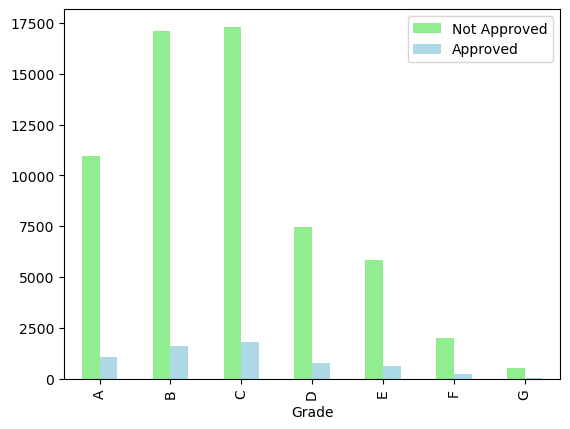
\includegraphics[width=8cm, height = 5.5cm]{images/grade vs loan status.png}
    \caption{Grade Bar Chart}
    \Description{Grade Bar Chart}
\end{figure}

After conducting a thorough analysis for \figurename{ 9}, it appears that there is no definitive relationship between grades, which is the reliability of the applicant and loan approval. While one might expect that borrowers with higher grades would be more likely to receive a loan, this does not always seem to be the case. To better understand the patterns at play, I compiled a detailed table that breaks down the values of the chart into percentages. By examining this data, we can begin to gain a deeper understanding of whether or not grades and loan status are truly correlated.

\begin{table}[h]
    \centering
    \caption{Percentages of Grades vs Loan Status}
    \label{tab:percentage of grades vs loan status}
    \begin{tabular}{|c|c|c|}
        \hline
        Loan status & Not Approved & Approved  \\
        \hline
        Grade       &              &           \\
        \hline
        \textbf{A}  & 90.8752\%    & 9.1248\%  \\
        \hline
        \textbf{B}  & 91.2763\%    & 8.7237\%  \\
        \hline
        \textbf{C}  & 90.6104\%    & 9.3896\%  \\
        \hline
        \textbf{D}  & 90.3620\%    & 9.6380\%  \\
        \hline
        \textbf{E}  & 90.4127\%    & 9.5873\%  \\
        \hline
        \textbf{F}  & 89.6260\%    & 10.3740\% \\
        \hline
        \textbf{G}  & 89.3651\%    & 10.6349\% \\
        \hline
    \end{tabular}
\end{table}

Analysising \tablename{ 1}, we can see that the percentages of approvals vs not approvals are extremely similar and hence,
it does not look like grades have a significant impact on loan approval. However, there are also subgrades, hence next, I am going to look at the
correlation between grade/subgrades and loan status to determine if there is a relationship or not.

\begin{figure*}
    \centering
    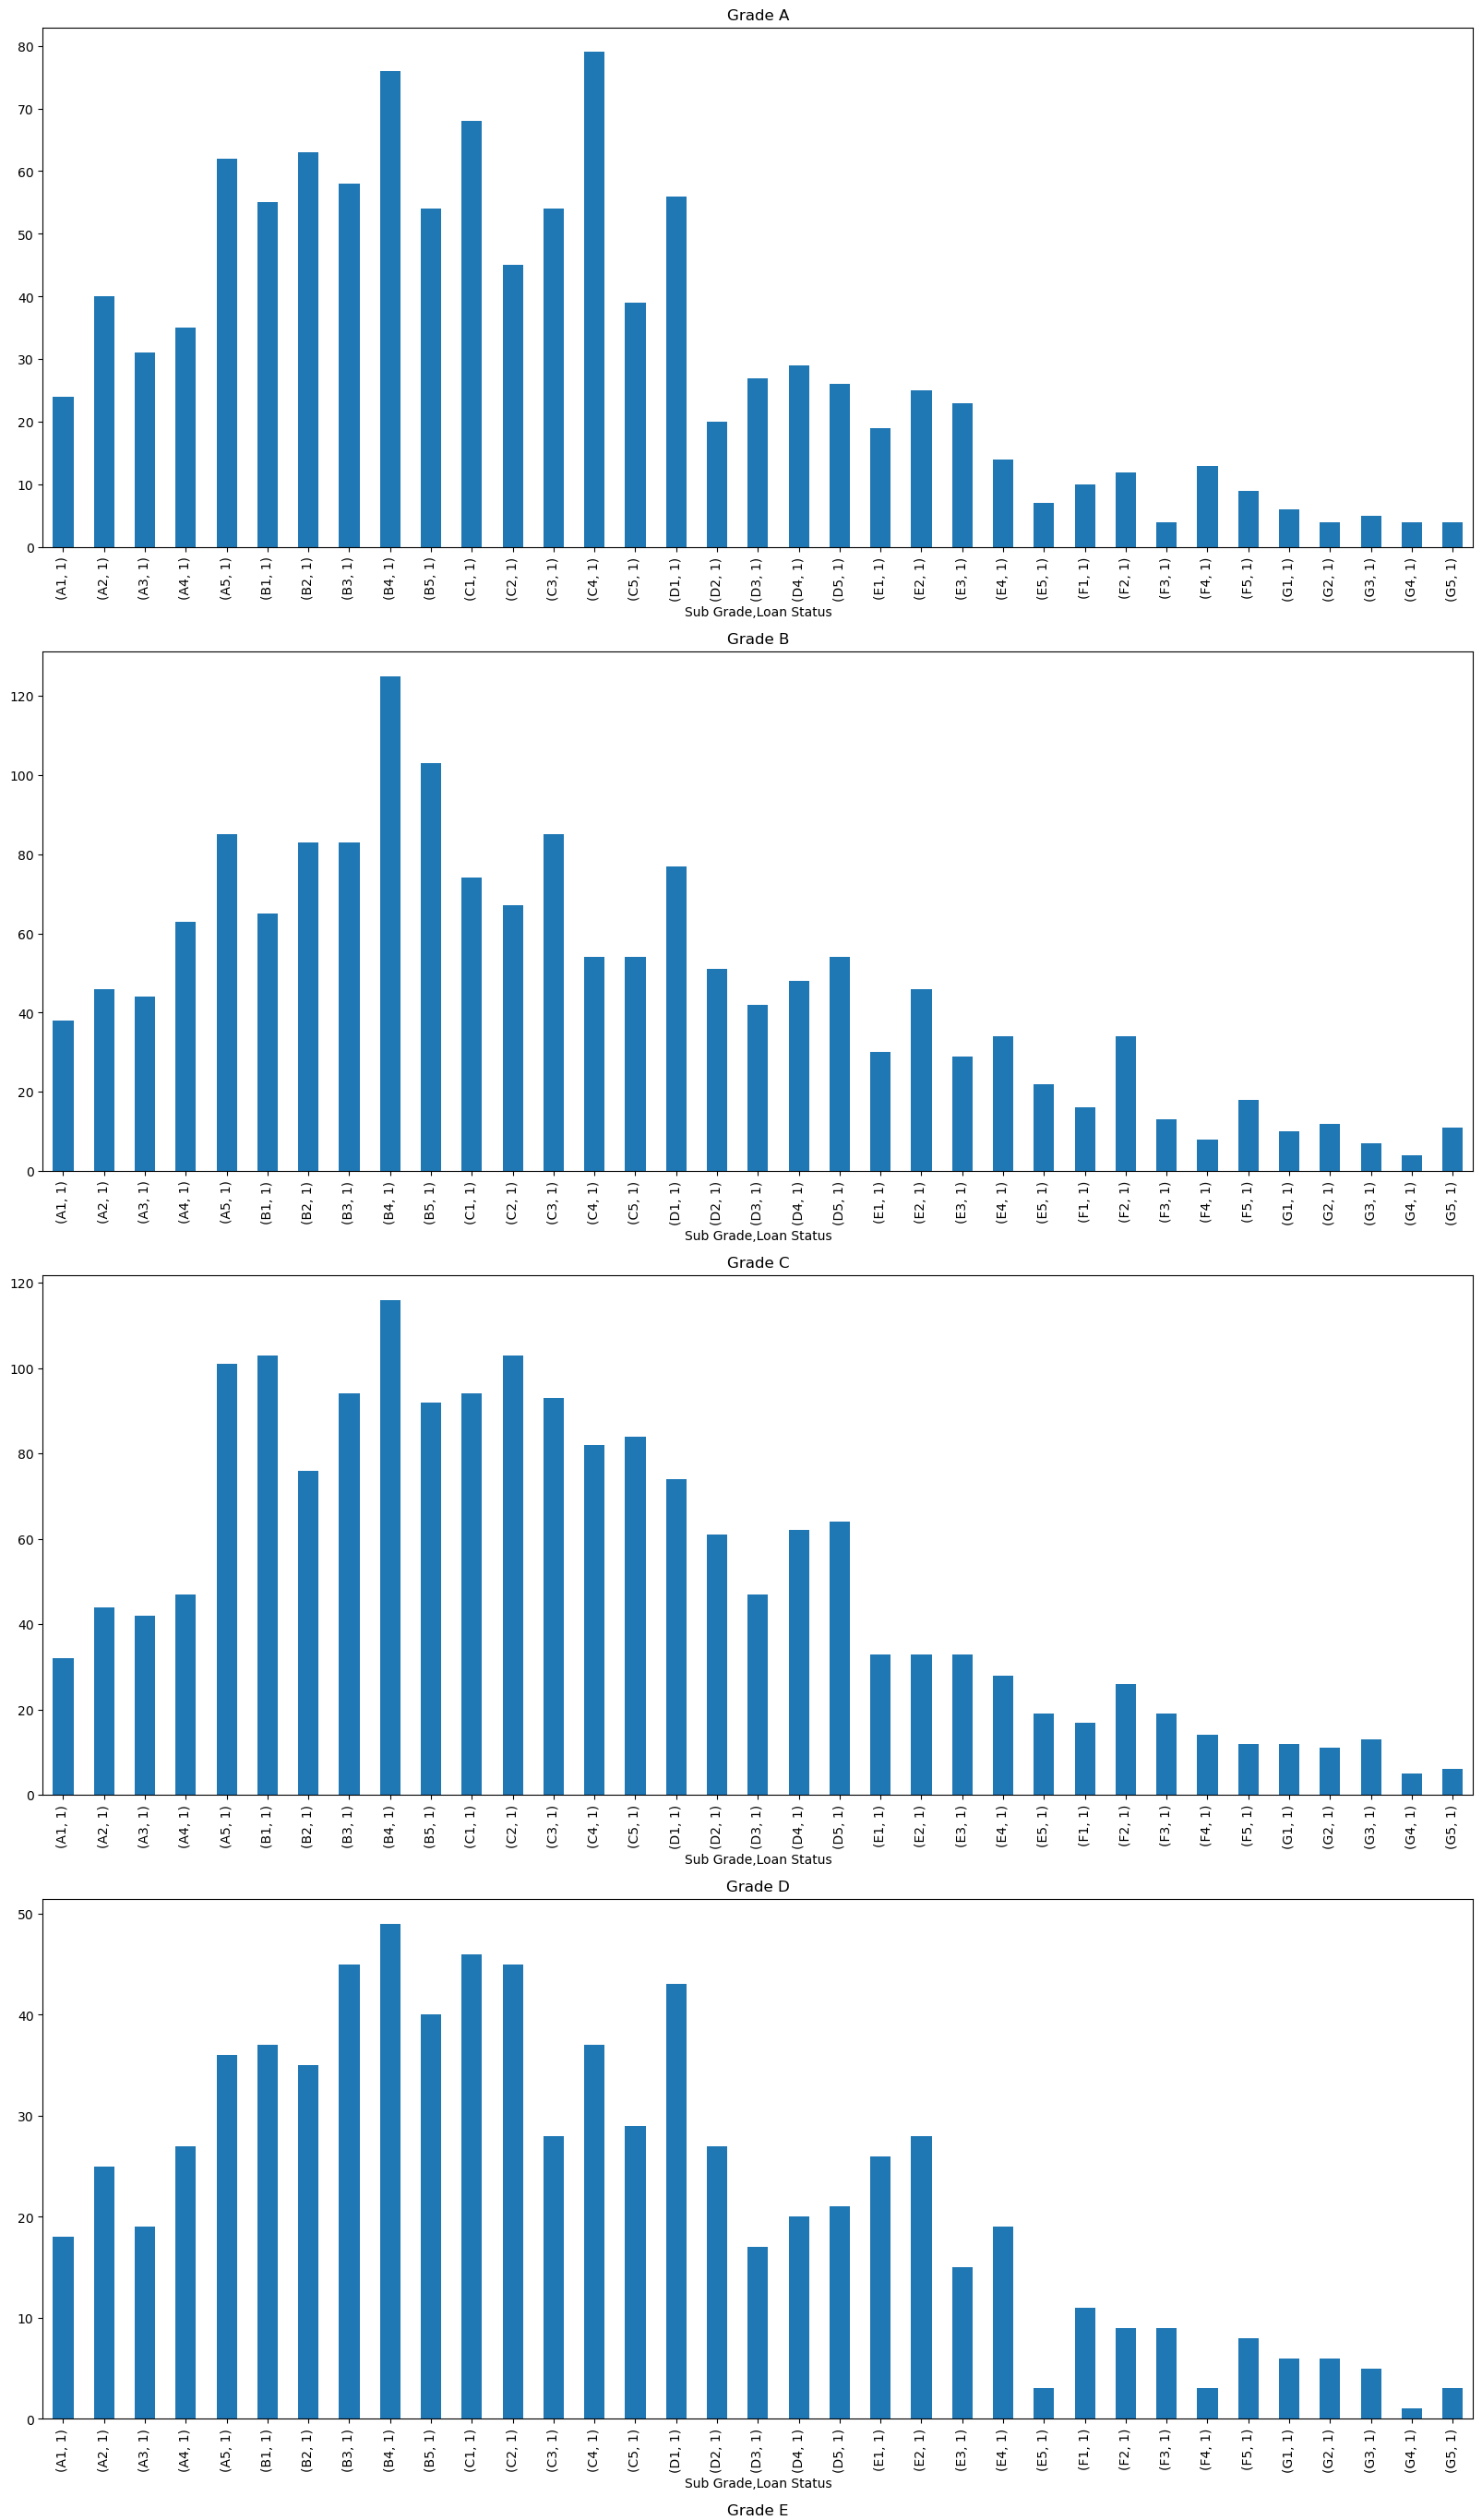
\includegraphics[width=\linewidth, height=\textheight]{images/grade-subgrade vs loan status-1.png}
    \caption{Grade Bar Chart}
    \Description{Grade Bar Chart 1}
\end{figure*}

\begin{figure*}
    \centering
    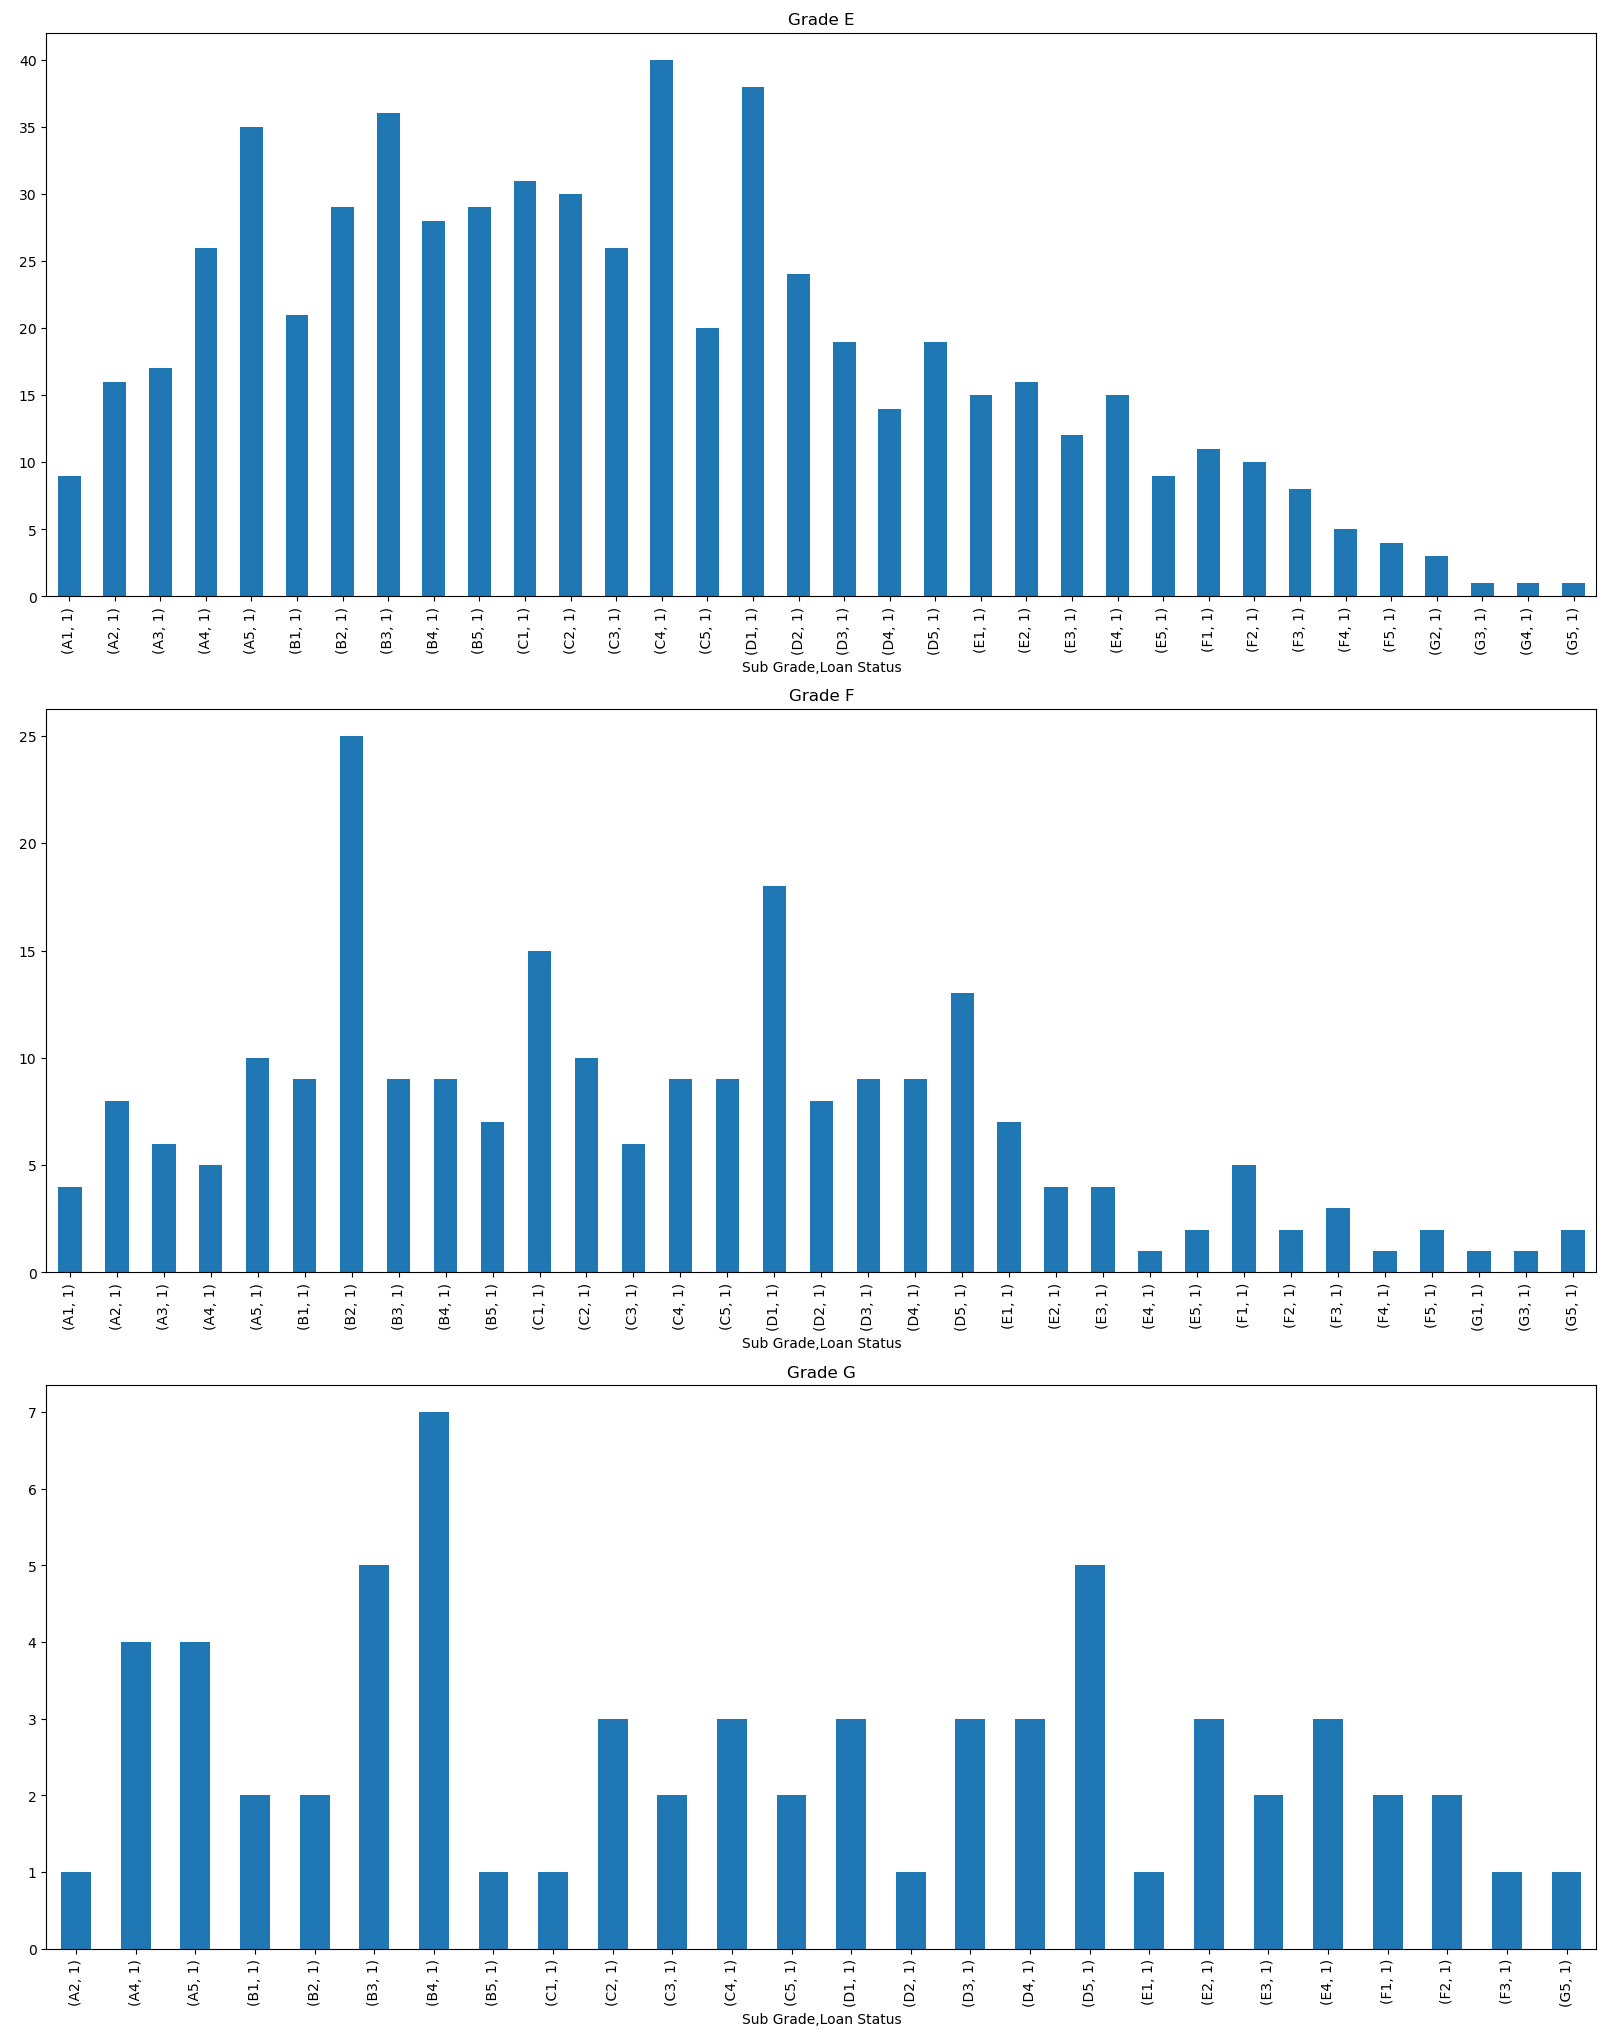
\includegraphics[width=\linewidth, height=\textheight]{images/grade-subgrade vs loan status-2.png}
    \caption{Grade Bar Chart}
    \Description{Grade Bar Chart 2}
\end{figure*}

Upon analyzing the distribution of grades and subgrades on \figurename{10 and 11} which are display on the next page, we can conclude that higher grades, particularly within the A, B, and C subsets, are more likely to be approved for loans. In fact, our data shows that A, B, and C grades have significantly more loan approvals than D, E, F, and G grades. While this suggests a correlation between the grade and loan approvals, it is important to note that other factors may also play a role in the decision-making process which dampened the affect of grade on the prediction enough to make the correlation unclear.

Furthermore, when we examined the subgrades, we found that there is a unimodal hump, right-skewed in the higher grades of A, B, and C. This means that the higher the grade, the greater the likelihood of loan approval. However, it is worth noting that this correlation is not always absolute, and there may be cases where a lower grade still results in loan approval.

Overall, these findings indicate that an applicant's grade does in fact play a factor in determining loan approval.

\begin{figure*}[h]
    \centering
    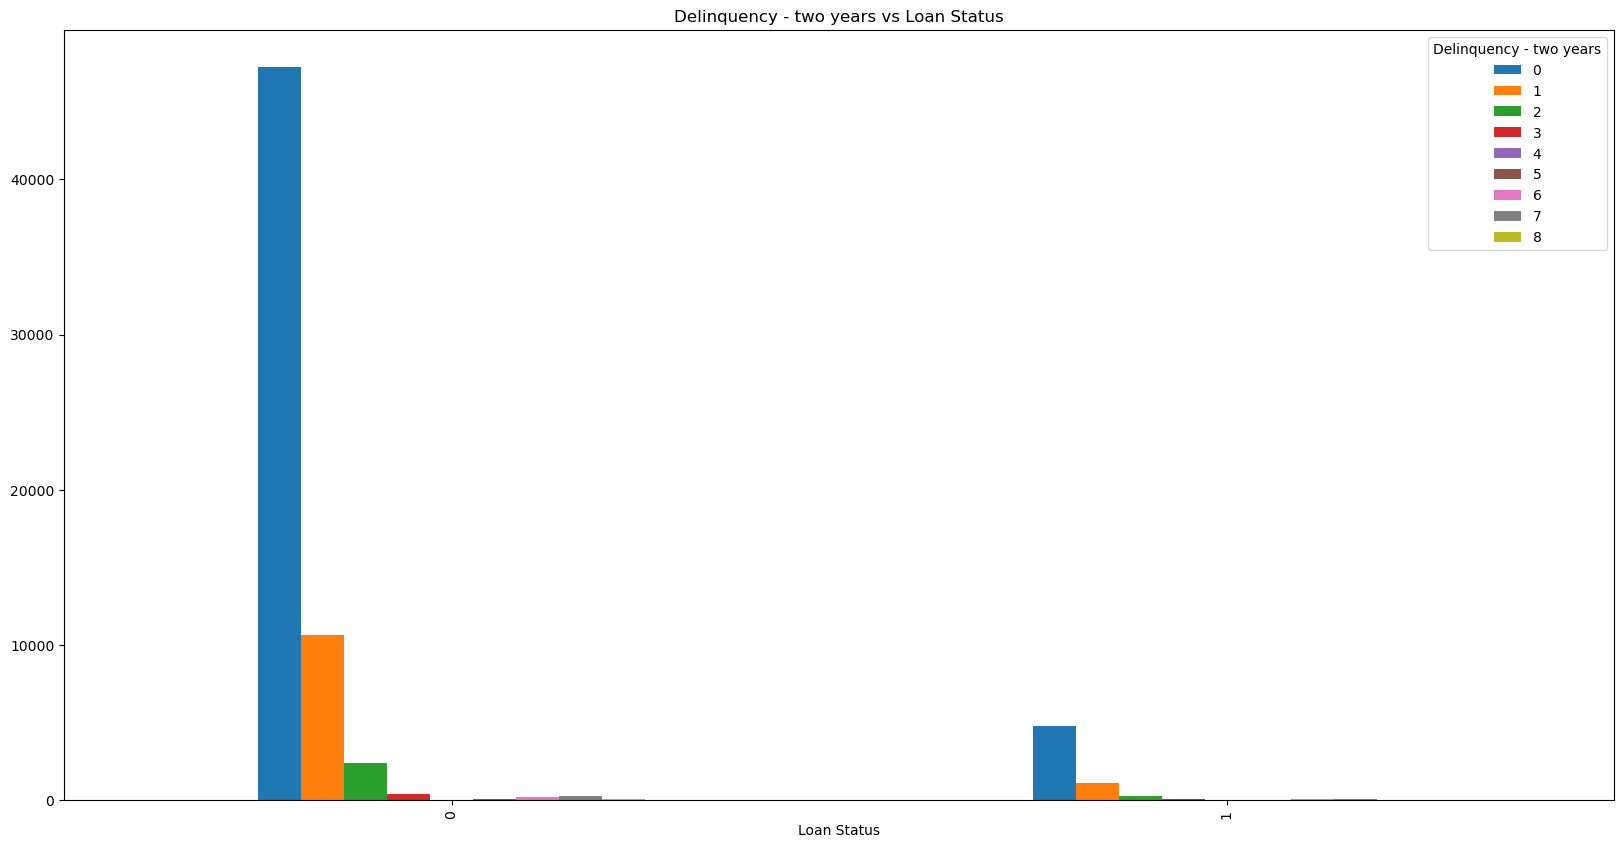
\includegraphics[width=\linewidth]{images/delinquency.png}
    \caption{Delinquency Bar Chart}
    \Description{Delinquency Bar Chart}
\end{figure*}
\begin{table*}[h]
    \centering
    \caption{Distributions of Delinquency vs Loan Status}
    \label{tab:percentage of Delinquency vs loan status}
    \begin{tabular}{|c|c|c|c|c|c|c|c|c|c|}
        \hline
        \text{Delinquency - two years}      & 0         & 1        & 2        & 3       & 4        & 5        & 6        & 7        & 8        \\
        \hline
        \text{Loan Status}                  &           &          &          &         &          &          &          &          &          \\
        \hline
        0                                   & 0.772222  & 0.173859 & 0.039136 & 0.00655 & 0.000212 & 0.001062 & 0.002679 & 0.003675 & 0.000604 \\
        1                                   & 0.765422  & 0.174972 & 0.040859 & 0.00705 & 0.000481 & 0.001442 & 0.004326 & 0.004326 & 0.001122 \\
        \text{Diff Approved - Not Approved} & -0.006800 & 0.001113 & 0.001723 & 0.00050 & 0.000268 & 0.000380 & 0.001647 & 0.000651 & 0.000517 \\
        \hline
    \end{tabular}
\end{table*}

\newpage

Next, let's examine "Delinquency - Two Year". We believe that this feature should have a decent correlation with loan approvals, as someone with a bad credit history should theoretically be less likely to get approved.
We plotted both a graph and a table in order to see if there are any underlying patterns / relationships between the features,

The graph and table both do not provide conclusive evidence of a correlation between the two features. Further research and analysis may be required to determine if there is a relationship. It is puzzling why a better history does not appear to increase the probability of an applicant being approved, as it seems reasonable to assume that it would. However, there could be various other factors that are not being accounted for in our analysis. Perhaps the sample size or the selection criteria have an impact on the correlation. Another possibility is that the data itself is incomplete or inaccurate.

Despite the lack of a clear correlation in the data, it is  we will continue to explore on this, and hopefully find out reasons as to why this is the outcome.

Another relationship we want to explore is between the "Total Revolving Credit Limit" and "Total Collection Amount." Both variables relate to the applicant's credit and can indicate the level of responsibility or irresponsibility a person has.

\begin{figure}[!h]
    \centering
    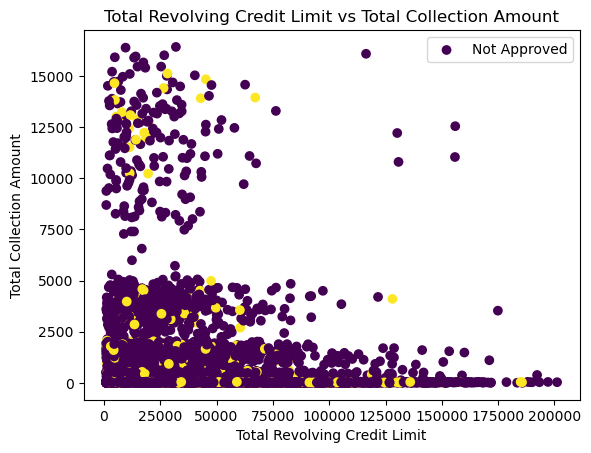
\includegraphics[width=\linewidth, height=6cm]{images/trclvstca.png}
    \caption{Total Revolving Credit Limit Bar Chart}
    \Description{Total Revolving Credit Limit Bar Chart}
    % reduce the padding between the figure and the caption
    \vspace{-1cm}
\end{figure}

Looking at the graph there is a slight correlation betweeh both the 'Total Revolving Credit Limit' and 'Total Collection Amount'.
Whereby, the as either of the values geet larger, the probability of the loan being approved decreases as the number of dots that
are not approved decreases as the values increase.

This again like all the data visualized in the EDA, is a weak correlation between the features and the target value, however, it is still enough of a correlation
both in the data and in a real world scenario to keep it for the model.


\section{Predictive Task}
After  identifying important features through exploratory data analysis, we will attempt to predict a person's loan status.
As this is a classification prediction problem. We will focus on decision tree classifiers, random forest classifiers, and other models.
\subsection{Evaluation}
We will use the F1-score metric as our evaluation method because our data is highly imbalanced between classes. This imbalance causes accuracy to be biased, and F1-score provides a better indication of whether our model is performing well or simply guessing the more common classification. The F1-score combines precision and recall into a single score, balancing both measures.

When working with imbalanced datasets, it is important to keep in mind that accuracy may not always provide a complete picture of a model's performance. This is because an imbalanced dataset has a disproportionate number of instances of one class compared to the other(s), which can skew results. While a model that classifies all instances as belonging to the majority class would achieve a high accuracy score, it would still be a poor model as it fails to take into account the minority class.

To better evaluate our model's performance in such cases, we can use the F1-score, which is a more comprehensive metric that balances both precision and recall. Unlike accuracy, the F1-score takes into account both false positives and false negatives. It measures the harmonic mean of precision and recall, providing a better indication of how well our model is performing on the minority class.

By using the F1-score, we can better assess whether our model is performing well or simply guessing the more common classification. This allows us to fine-tune the model to better handle the imbalanced dataset and improve its performance on the minority class.

\subsection{Model Evaluation/Baseline}
\begin{figure}[b]
    \centering
    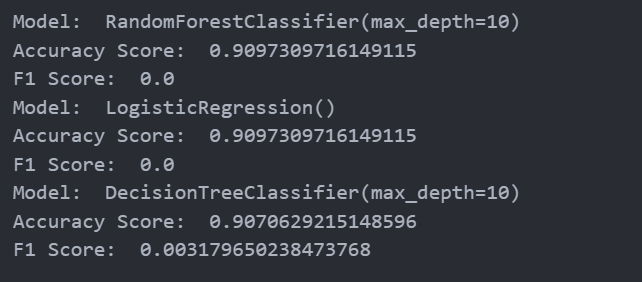
\includegraphics[width=\linewidth]{images/baseline.png}
    \caption{Baseline Model Comparison}
    \Description{Baseline Model Comparison}
\end{figure}

For our Baseline model, we are using four models as a baseline: Logistic Regression, K-Means Clustering, Decision Tree Classification, and Random Forest Classification.

To deal with the categorical variables, we will perform basic one-hot encoding and leave all the numerical variables as they are.

\subsubsection{Logistic Regression}
This model assumes a linear relationship between the features and the label (loan status). Looking at the performance of this model, we can see that it achieved an accuracy of over 90\\%. However, as we discussed earlier, accuracy is a poor metric to determine the performance for this dataset as the dataset is highly imbalanced. Hence, the F-1 score is a more important metric to look at for this model.

For the F1-score, we got a 0, indicating that the model only predicted 0s and did not predict any 1s, which gave us the high accuracy score. This is a clear indication that the model is not performing well and needs to be improved, or we should use a different model.

\subsubsection{Decision Tree Classifier}
This is a non-parametric supervised learning algorithm that can be used for both classification and regression tasks. Decision trees break down complex data into more manageable parts. They can automatically handle missing values, capture non-linear relationships, and are suitable for both numerical and categorical data.

After testing this model on our imbalanced dataset, we obtained an F-1 score of 0.0016, which is better than that obtained with Logistic Regression, while still maintaining a relatively similar accuracy score.

\subsubsection{Random Forest Classifier}
Random forests, also known as random decision forests, are an ensemble learning method used for classification, regression, and other tasks. During training time, they construct numerous decision trees. Random forests may overfit the data, but there are ways to optimize them and prevent overfitting.
The F-1 score for this model on our imbalanced dataset is 0, which does not make sense as Decision Tree managed to get a score of 0.0032. Our suspicion for this is that the model is overfitting the data. We will try to optimize the model to see if we can improve the F-1 score.

All baseline models are fitted on the same training set, and all hyperparameters are set to their default values to test the model's basic performance.

\subsection{Conclusion}
After analyzing the models above, we have decided to focus on Decision Trees and Random Forest Classifiers. As due to the extreme randomness and lack of correlation between the features, we think that the complexity and the ability to solve non-linear problems may be beneficial to our model. Our goal is to perform feature engineering to improve the F1-score and reduce the noise in the data, choose the optimal hyperparameters to improve our models, and fine-tune the models to select our final model.

\section{Feature Engineering}
\subsection{Ordinal Encoding}
We are combining the "Grade" and "Sub Grade" columns to create a new column called "GradeSubGrade." Since these grade categories are ordinal, we prefer ordinal encoding over one-hot encoding or any other encoding methods. For example, the grade AF1 is worse than grade AA1. This also makes the model more efficient by reducing memory (number of columns in one-hot encoding) and increasing speed.

This was done by combining the grades and subgrades into a single column, then getting all the unique grades and sorted them in ascending order.
Which we then used to map the grades to numbers.
\begin{minted}{python}
grade = train["Grade"].unique()
subgrade = train["Sub Grade"].unique()
train["GradeSubGrade"] = 
    train["Grade"] + train["Sub Grade"]
train = train.drop(
    columns= ["Grade", "Sub Grade"]
)

features = []

for i in grade:
    for j in subgrade:
        lst = [i+j]
        features.append(lst)
features = np.unique(features)

dicta = {}
k = 1
for i in features:
    dicta[i] = k
    k = k+1

train["GradeSubGrade"] = 
    train["GradeSubGrade"].replace(dicta)
\end{minted}

\subsection{Unbalanced Dealing}
Since this dataset is highly unbalanced, we have decided to balance it by under-sampling. In real-world scenarios, loan statuses are not equally likely to be defaulted. Therefore, we try to keep the percentage divide unequal yet close. We run a test and choose the optimal balanced set.

\begin{minted}{python}
zeros = train.loc[
    train["Loan Status"] == 0
    ]
ones =  train.loc[
    train["Loan Status"] == 1
    ]

balanced = zeros.sample(ones.shape[0])
balanced_df = pd.concat(
    [ones, balanced], axis = 0
    ).reset_index()
balanced_df = balanced_df.drop(
    columns = ["index"]
    )
\end{minted}

\subsection{One-Hot Encoding}
One-hot encoding is a machine learning technique used to convert categorical information into a format that can be fed into machine learning algorithms to improve prediction accuracy. In this document, we are using one-hot encoding for categorical features such as "Employment Duration," "Verification Status," "Application Type," "Delinquency - two years," and "Collection 12 months Medical." Since these features are not in any specific order and cannot be classified as ordinal, we are choosing one-hot encoding over other encoding methods.

This was done using sklearn column transformer and one-hot encoder.
\begin{minted}{python}
preproc = ColumnTransformer([
(
    "One-hot", OneHotEncoder(), 
    [
     "Employment Duration", "Verification Status", 
     "Application Type", "Delinquency - two years", 
     "Collection 12 months Medical"
    ]
)
\end{minted}


\subsection{Standard Scaling}
Standard scaling is a common data pre-processing technique used in machine learning to transform data into a standard format. It scales the features of a dataset so that they have a mean of zero and a standard deviation of one. This is achieved by subtracting the mean of each feature from each observation and then dividing the result by the standard deviation of that feature.

Standard scaling is useful when working with datasets where the features have different units or scales. It is also useful when features have a very wide range (for example, 0 to 1,000,000). Failure to account for these differences in scale may lead to biased results, as some features may dominate others in the analysis. Standard scaling helps to mitigate this problem by ensuring that all features are on the same scale. In this study, we chose to use standard scaling for the "Total Collection Amount" and "Total Received Late Fee" features because their ranges are wide, and their distributions are very skewed. The code for standard scaling is provided below.
\begin{minted}{python}
    (
        "Std-scale", StandardScaler(),
         ['Total Collection Amount',
          'Total Received Late Fee']
    )
], remainder="passthrough")
\end{minted}

\section{Final Model}
\subsection{Parameter Hypertuning}
First we took all the engineered features  and split them into training and testing sets and a $\textbf{Random\_State = 42}$ to prevent any randomness so
that we can get the same results every time we run the code and to get a fair comparison between the models. Which we then used GridSearchCV to find the optimal hyperparameters for our model.

\begin{minted}{python}
X = balanced_df.drop(
    'Loan Status', axis=1
)
y = balanced_df['Loan Status']

X_train, X_test, y_train, y_test = 
train_test_split(X, y, test_size=0.2, random_state=42)

rf_pipe = Pipeline([
("preprocessing", preproc),
("rf", rf)
])

param_grid = {
'rf__n_estimators' : [10, 30, 50, 75, 100],
'rf__max_depth' : [2, 5, 10, 20, None],
'rf__min_samples_split' : [1, 2, 5, 10],
'rf__class_weight' : [
    "balanced", 
    "balanced_subsample",
    None
    ]
}

grid_search_rf = GridSearchCV(rf_pipe, 
    param_grid=param_grid, cv=5, 
    scoring='f1', n_jobs=-1, verbose=1
    )

grid_search_rf.fit(X_train, y_train)
\end{minted}

We also did the same thing for the Decision Tree Classifier:
\begin{minted}{python}
dt_pipe = Pipeline([
("preprocessing", preproc),
("dt", dt)
])

param_grid = {
    'dt__max_depth' : [2, 5, 10, 20, None],
    'dt__min_samples_split' : [1, 2, 5, 10],
    'dt__class_weight' : ["balanced", None]
}

grid_search_dt = GridSearchCV(
    dt_pipe, param_grid=param_grid,
     cv=5, scoring='f1', n_jobs=-1, verbose=1
)

grid_search_dt.fit(X_train, y_train)
\end{minted}

This gave us the following results:

\begin{table}[h]
    \centering
    \begin{tabular}{|c|p{4cm}|}
        \hline
        Param          & Value                                                                                                                       \\
        \hline
        RF Best Params & $\{$'rf\_\_class\_weight': 'balanced', 'rf\_\_max\_depth': 2, 'rf\_\_min\_samples\_split': 10,'rf\_\_n\_estimators': 10$\}$ \\
        \hline
        RF Best Score  & 0.5022874168816818                                                                                                          \\
        \hline
        DT Best Params & $\{$'dt\_\_class\_weight': 'balanced',
        'dt\_\_max\_depth': None,
        'dt\_\_min\_samples\_split': 10$\}$                                                                                                          \\
        \hline
        DT Best Score  & 0.5102653441988605                                                                                                          \\
        \hline
    \end{tabular}
\end{table}

We can see that both the Random Forest and Decision Tree Classifier have scores that are really similar, with Decision Tree beating out
the Random Forest out by a small margin, which could easily be due to Random Chance, hence moving into feature selection, we are going to
continue to use both the Random Forest andd Decision Tree.

\newpage
\section{Literature}
\subsection{Jay Dixit's Analysis}
\href{https://www.kaggle.com/code/jayrdixit/loan-default-prediction}{Link to Jay Dixit's Analysis}

Our project was inspired by a Kaggle project on Loan Defaults, which aimed to predict whether a loan applicant is likely to default. The original analysis, performed by Jay Dixit, involved data exploration, cleaning, pre-processing, feature engineering, and building machine learning models. Jay used various techniques, including data visualization, correlation analysis, and feature selection, to identify the most important features for the models. Our approach differed in some respects. For example, we used ordinal encoding rather than normalization to encode the “Grade” and “Sub-Grade” columns, and we balanced the dataset due to the highly imbalanced class distribution.

In contrast to Jay's analysis, we used Logistic Regression, Random Forest Classifier, and Decision Tree Classifier with default parameters to create baseline models. Our final model focused on the Random Forest Classifier, for which we performed Grid Search CV to identify the optimal hyperparameters with the best F1 score. The final model achieved an F1 score of 0.51 on the test data, significantly higher than the baseline models. This result demonstrates the efficacy of our approach, which included feature engineering, hyperparameter tuning, feature selection, and model optimization.

\subsection{Ann Mary's Analysis}
\href{https://www.kaggle.com/code/annmary25/loan-status-prediction}{Link to Ann Mary's Analysis}

A related task has been undertaken by various researchers on different datasets. In particular, Ann Mary's report on Kaggle examines a dataset containing personal and financial information of loan applicants to predict loan approval. It is worth noting that the dataset utilized by Ann Mary contains more comprehensive information about an applicant's personal characteristics, such as gender and age.

The author of the report employed various techniques, including oversampling the minority class and hyperparameter tuning, to improve the performance of the models. The best performing model was a Random Forest Classifier, which achieved remarkable results.

Overall, the report provides valuable insights into predicting loan statuses and highlights the efficacy of machine learning models in addressing this challenge. This motivated us to find a more comprehensive dataset and refine our approach to this problem. As a result, we were able to train and optimize a model that accurately predicts whether an individual will default on a loan.

\section{Conclusion}
\subsection{Results Comparison}
After balancing the dataset and performing feature engineering, we were able to improve the F1-score from 0.003 to 0.605, which is a significant improvement over the baseline model. However, our accuracy decreased to 0.5146175410492592. This is because the dataset is now balanced, and we are no longer just predicting the majority class, which would have resulted in a high accuracy.

We also calculated the confusion matrix, we noticed that our model is predicting more 1's than 0's. This indicates a bias that could be caused by several factors:

\begin{itemize}
    \item  Features: The features we used to train our model might be more indicative of class 1 than class 0, leading to a bias towards class 1.
    \item  Model complexity: It is possible that the model is too complex, resulting in overfitting and more 1's being predicted than 0's.
    \item  Data quality: The data we used may contain errors or biases that are affecting the model's predictions.
\end{itemize}

\subsection{Resuts Evaluation}
However, I do still think that the model is not the best model for predicting loans. This is because with a balanced dataset, and getting approximately
50\% accuracy, there might be a chance that the model is predicting the results 50/50 which could also be a problem to look into.

\subsection{Final Words}
After balancing the dataset and performing feature engineering, we were able to significantly improve the F1-score from 0.003 to 0.605 over the baseline model. However, our accuracy decreased to 0.5146175410492592. This is because the dataset is now balanced, and we are no longer simply predicting the majority class, which would have resulted in a high accuracy.

In our opinion, while the dataset we chose may be good, it may not be the best choice for modeling and predicting credit loans. This is because the correlations between the features are relatively weak, indicating that the dataset contains too much noise and randomness to predict accurate results with certainty.

However, there could be multiple reasons for this. Firstly, as the dataset was taken from Kaggle, it is possible that the true source of the dataset is not reliable or accurate. This is supported by the fact that during our exploratory data analysis, there was no clear-cut correlation between the features and the target variable. Therefore, it may be necessary to look for other sources of data, or to apply more advanced techniques to clean and preprocess the data before modeling.

Moreover, it is important to consider the potential impact of the data quality on the model performance. Inaccurate or incomplete data can lead to biased or inaccurate predictions, which can have serious consequences in the context of credit loans. Therefore, it is crucial to carefully evaluate the quality and relevance of the data before using it for modeling, and to continuously monitor and improve the data quality throughout the modeling process.

Secondly it is also possible that there were other factors that were not accounted for in our analysis. It is possible that we did not choose the best features or methods to predict loans, despite our best efforts to utilize our knowledge and available tools for feature engineering, selecting models, and evaluating our results. We are continuing to explore and fine-tune our models to improve accuracy and reduce noise in the data.

Thirdly, it could be that loan approvals in the real world are heavily biased by the loan approver, or that many approved loans are based more on the loaner's decision than the true statistics of the applicant. This introduces a lot of noise into the dataset, making it difficult to predict the outcome.

Overall, there may be many other reasons why our model can only predict loans with moderate accuracy. However, given the time and the resources we had, we believe we did everything we could to produced a model that can predict loans with reasonable accuracy and a good F1-score.

\section{References}
Jay Dixit Kaggle -
\href{https://www.kaggle.com/code/annmary25/loan-status-prediction}{Link to Kaggle}

Ann Mary Kaggle -
\href{https://www.kaggle.com/code/jayrdixit/loan-default-prediction}{Link to Kaggle}


\section{Github repository}


\section{Working Demo}
To use the working demo of the project, please follow the steps below:

\begin{itemize}
    \item Download the project from the Github repository.
    \item cd into the webapp directory.
    \item Run the python script in app.py
    \item Webapp should be runnnig on localhost
\end{itemize}

\end{document}